\documentclass[12pt,a4paper]{article}

\usepackage[T2A]{fontenc}
\usepackage[utf8]{inputenc}
\usepackage[english,russian]{babel}
\usepackage{geometry}
\usepackage{graphicx}
\usepackage{float}
\usepackage{caption}
\usepackage{array}
\usepackage{booktabs}
\usepackage{longtable}
\usepackage{tabularx}
\usepackage{enumitem}
\usepackage{tikz}
\usepackage{xcolor}
\usepackage{hyperref}
\usepackage{fancyhdr}

\usetikzlibrary{arrows.meta,positioning,shapes.geometric}
\geometry{left=2.5cm,right=1.5cm,top=2cm,bottom=2cm}
\graphicspath{{docs/screenshots/}}
\hypersetup{colorlinks=true,linkcolor=black,urlcolor=blue,
  pdftitle={Отчёт по лабораторной работе №2},
  pdfauthor={Цыканов Артём Эдуардович}}
\setlength{\parindent}{1.25cm}
\setlength{\parskip}{0.25em}
\captionsetup{font=small,labelfont=bf}
\pagestyle{fancy}
\fancyhf{}
\fancyhead[L]{Лабораторная работа №2}
\fancyhead[R]{Расширенный AI-сервис}
\fancyfoot[C]{\thepage}
\setlength{\headheight}{15pt}
\newcolumntype{Y}{>{\raggedright\arraybackslash}X}
\newcommand{\code}[1]{\texttt{#1}}

\begin{document}

\begin{titlepage}
  \begin{center}
    \textbf{МИНИСТЕРСТВО НАУКИ И ВЫСШЕГО ОБРАЗОВАНИЯ\\РОССИЙСКОЙ ФЕДЕРАЦИИ}
    \vspace{0.5cm}

    Федеральное государственное автономное образовательное учреждение\\
    высшего образования
    \vspace{0.3cm}

    \textbf{«НАЦИОНАЛЬНЫЙ ИССЛЕДОВАТЕЛЬСКИЙ\\
    ТЕХНОЛОГИЧЕСКИЙ УНИВЕРСИТЕТ «МИСИС»»}
    \vspace{1.5cm}

    \textbf{Институт компьютерных наук}\\[0.3cm]
    \textbf{Кафедра инженерной кибернетики}
    \vspace{1.7cm}

    \textbf{ЛАБОРАТОРНАЯ РАБОТА №2}\\[0.4cm]
    по дисциплине «Современные интеллектуальные сетевые сервисы»
    \vspace{1.5cm}

    {\Large\bfseries Расширение AI-сервиса:\\
    request ID, SQLite, batching и LLM}
  \end{center}
  \vfill
  \begin{flushright}
    \begin{tabular}{@{}ll@{}}
      Выполнил: & студент группы МПИ-25-1-1 \\
                & Цыканов Артём Эдуардович \\[0.5cm]
      Проверила: & Корнет Мария Евгеньевна
    \end{tabular}
  \end{flushright}
  \vfill
  \begin{center}Москва, 2026\end{center}
\end{titlepage}

\tableofcontents
\newpage

\section{Цель работы}

Расширить REST API сервиса агроскоринга: обеспечить трассировку запросов,
асинхронное хранение результатов, пакетный инференс, управление потоком
запросов, таймауты, пагинацию и безопасное подключение внешней LLM.

\section{Архитектура сервиса}

Каждый запрос проходит через middleware, которое формирует сквозной
\code{request\_id} и измеряет время выполнения. Pydantic и сервисный слой
проверяют данные, после чего запрос направляется в одиночный, явный пакетный
либо динамический пакетный контур инференса. Результаты сохраняются в SQLite.
Для LLM используется общий асинхронный HTTP-клиент.

\begin{figure}[H]
  \centering
  \resizebox{\textwidth}{!}{%
  \begin{tikzpicture}[
    node distance=7mm,
    block/.style={draw,rounded corners,align=center,minimum height=11mm,
                  minimum width=22mm,fill=blue!6},
    storage/.style={draw,cylinder,shape border rotate=90,aspect=0.25,
                   align=center,minimum height=14mm,fill=green!8},
    arrow/.style={-{Latex[length=2.3mm]},thick}]
    \node[block] (client) {Клиент};
    \node[block,right=of client] (middleware) {Middleware\\request ID};
    \node[block,right=of middleware] (api) {FastAPI};
    \node[block,right=of api] (validation) {Валидация};
    \node[block,above right=of validation] (single) {Single};
    \node[block,right=of validation] (batch) {Explicit\\batch};
    \node[block,below right=of validation] (queue) {Queue +\\worker};
    \node[block,right=18mm of batch] (engine) {Model\\engine};
    \node[storage,right=of engine] (db) {SQLite};
    \node[block,below=of engine] (llm) {Vireonix\\LLM};
    \draw[arrow] (client)--(middleware);
    \draw[arrow] (middleware)--(api);
    \draw[arrow] (api)--(validation);
    \draw[arrow] (validation)--(single);
    \draw[arrow] (validation)--(batch);
    \draw[arrow] (validation)--(queue);
    \draw[arrow] (single)--(engine);
    \draw[arrow] (batch)--(engine);
    \draw[arrow] (queue)--(engine);
    \draw[arrow] (engine)--(db);
    \draw[arrow] (api.south) |- (llm.west);
  \end{tikzpicture}}
  \caption{Компонентная схема расширенного AI-сервиса}
  \label{fig:architecture}
\end{figure}

Lifespan FastAPI инициализирует SQLite, модель, ограниченную очередь,
batch-worker и \code{httpx.AsyncClient}. При остановке worker отменяется, а
HTTP-клиент корректно закрывается. Исходный код находится в
\href{https://github.com/Artem216/siss/tree/main/lab_02}{репозитории на GitHub}.

\section{Реализованный API}

\begin{longtable}{>{\ttfamily\raggedright\arraybackslash}p{5.2cm}
                  >{\centering\arraybackslash}p{1.4cm}
                  >{\raggedright\arraybackslash}p{9cm}}
  \caption{Endpoints расширенного сервиса}\label{tab:endpoints}\\
  \toprule
  \normalfont\textbf{Endpoint} & \textbf{Метод} & \textbf{Назначение} \\
  \midrule\endfirsthead
  \toprule
  \normalfont\textbf{Endpoint} & \textbf{Метод} & \textbf{Назначение} \\
  \midrule\endhead
  \bottomrule\endfoot
  /health & \normalfont GET & \normalfont Проверка состояния API \\
  /model-info & \normalfont GET & \normalfont Информация о модели \\
  /predict & \normalfont POST & \normalfont Одиночный инференс и запись в SQLite \\
  /batch-predict & \normalfont POST & \normalfont Explicit batch до восьми объектов \\
  /predict-queued & \normalfont POST & \normalfont Dynamic batching через очередь \\
  /queue-status & \normalfont GET & \normalfont Состояние и настройки очереди \\
  /predictions & \normalfont GET & \normalfont История прогнозов и фильтрация \\
  /predictions/\{request\_id\} & \normalfont GET & \normalfont Один прогноз; 409 для batch \\
  /requests/\{request\_id\}/predictions & \normalfont GET & \normalfont Все элементы batch-запроса \\
  /predictions/by-weekday & \normalfont GET & \normalfont Пагинация по дню недели \\
  /demo/seed-weekdays & \normalfont POST & \normalfont Демонстрационные данные \\
  /llm/chat & \normalfont POST & \normalfont Запрос к OpenAI-совместимой LLM \\
  /predict-with-llm & \normalfont POST & \normalfont Скоринг и объяснение LLM \\
\end{longtable}

Ошибки возвращаются в едином формате с полями \code{detail} и
\code{request\_id}. Реализованы коды 400, 404, 409, 422, 429, 500, 502, 503 и
504. Заголовки каждого ответа содержат \code{X-Request-ID} и
\code{X-Process-Time}.

\section{Результаты работы}

\begin{figure}[H]
  \centering
  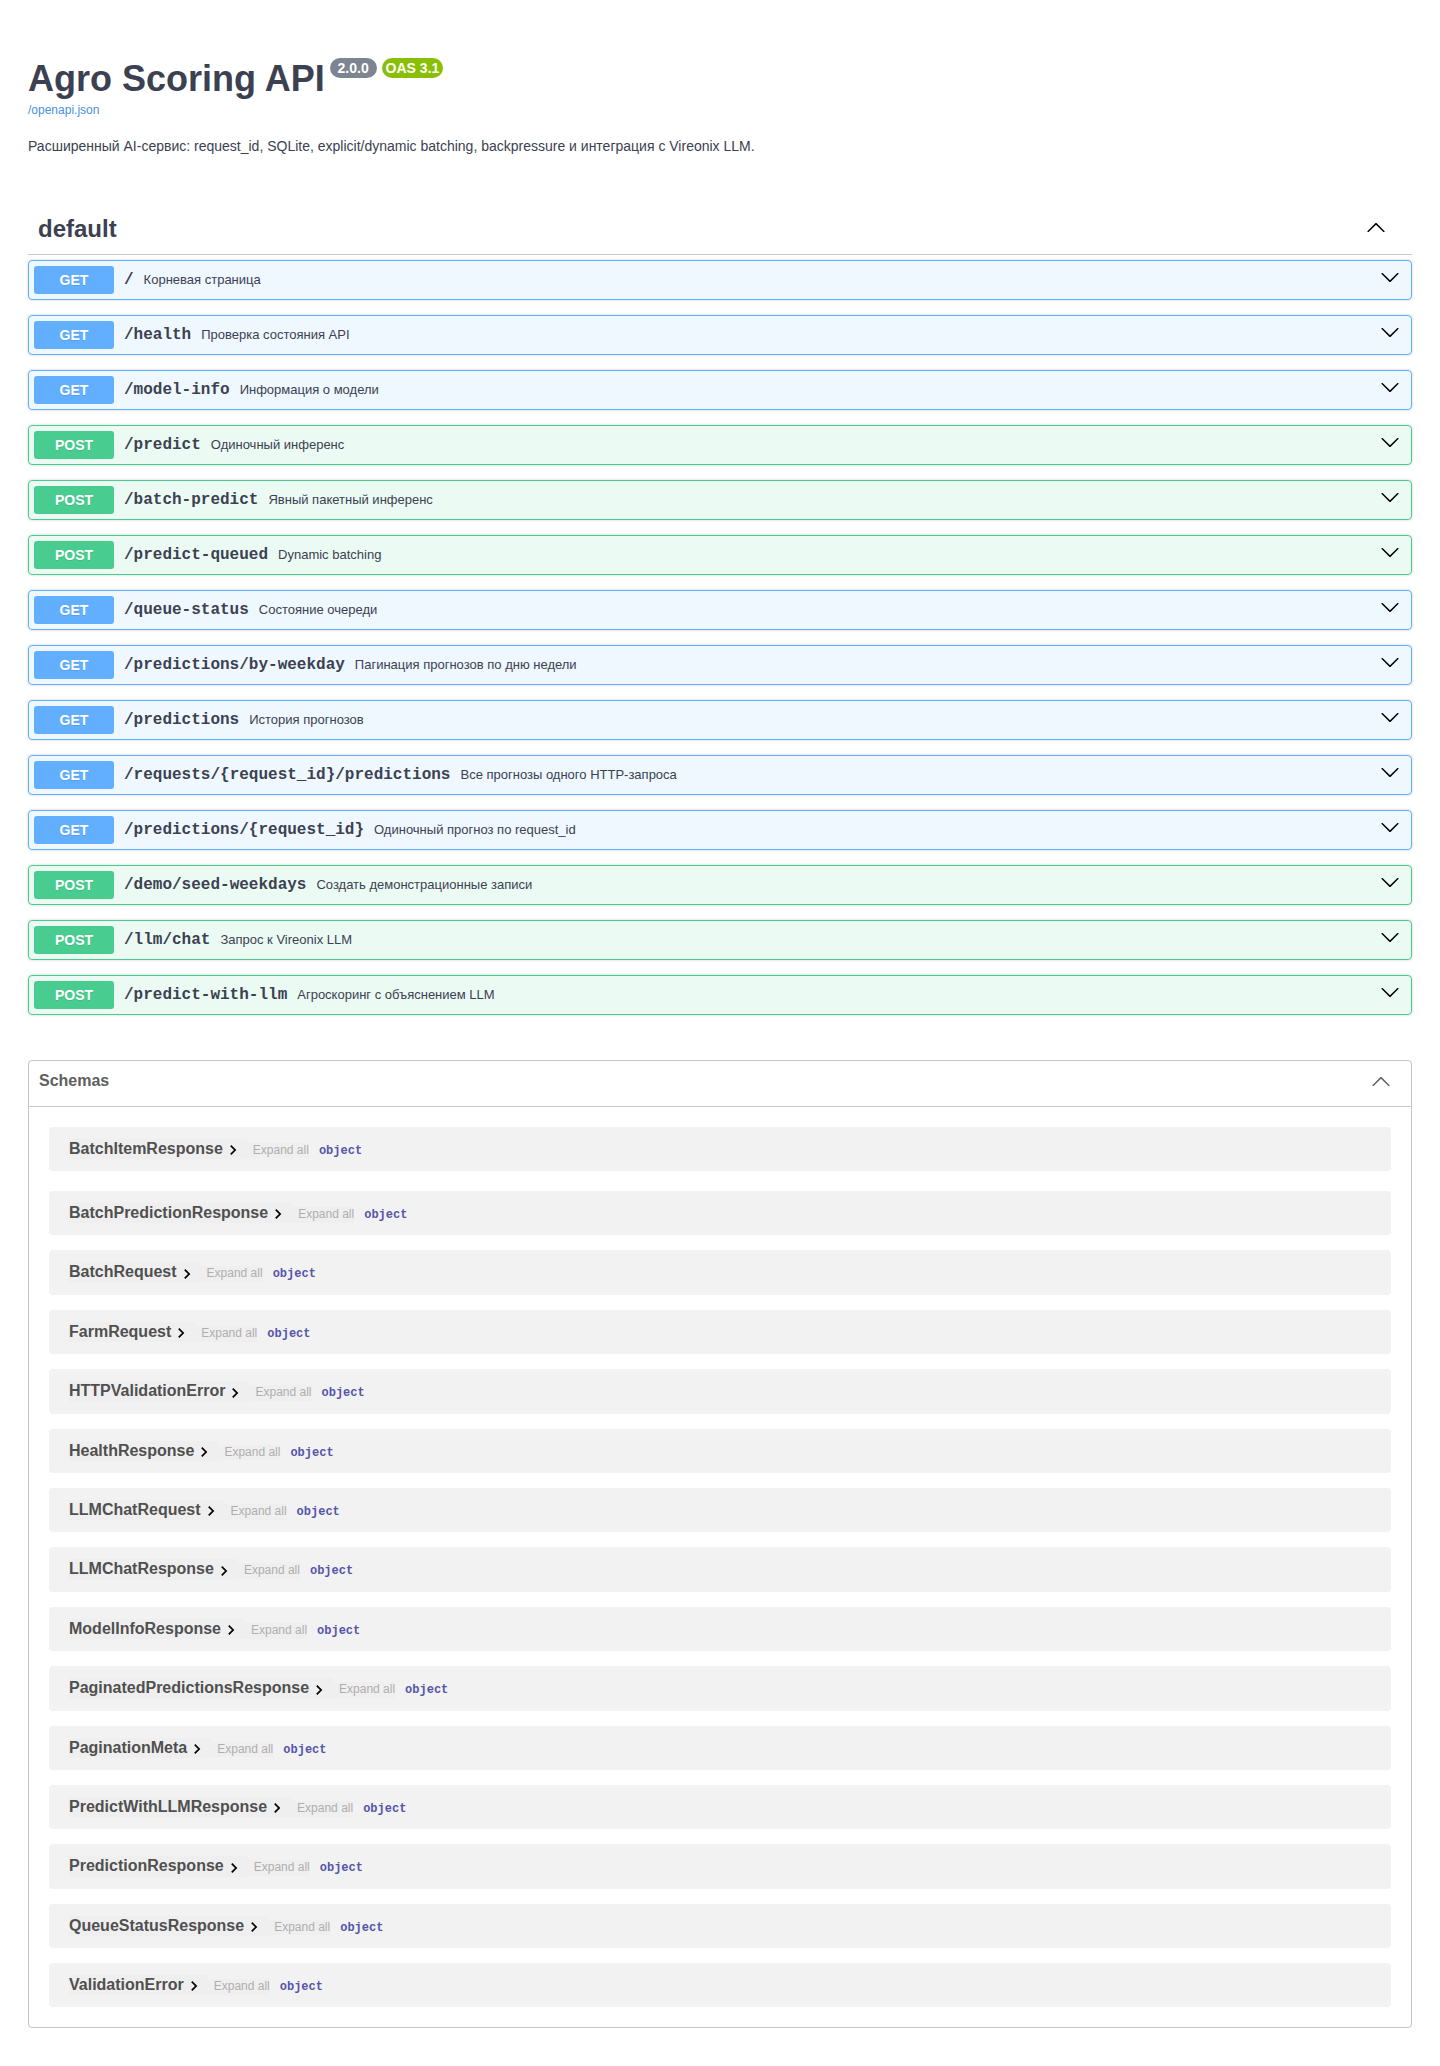
\includegraphics[width=\textwidth,height=.78\textheight,keepaspectratio]{swagger-ui.png}
  \caption{Документация Swagger UI}
\end{figure}

\subsection{Одиночный инференс и SQLite}

Клиент получает 200 только после успешного \code{COMMIT}. История читается из
SQLite в обратном порядке создания.

\begin{figure}[H]
  \centering
  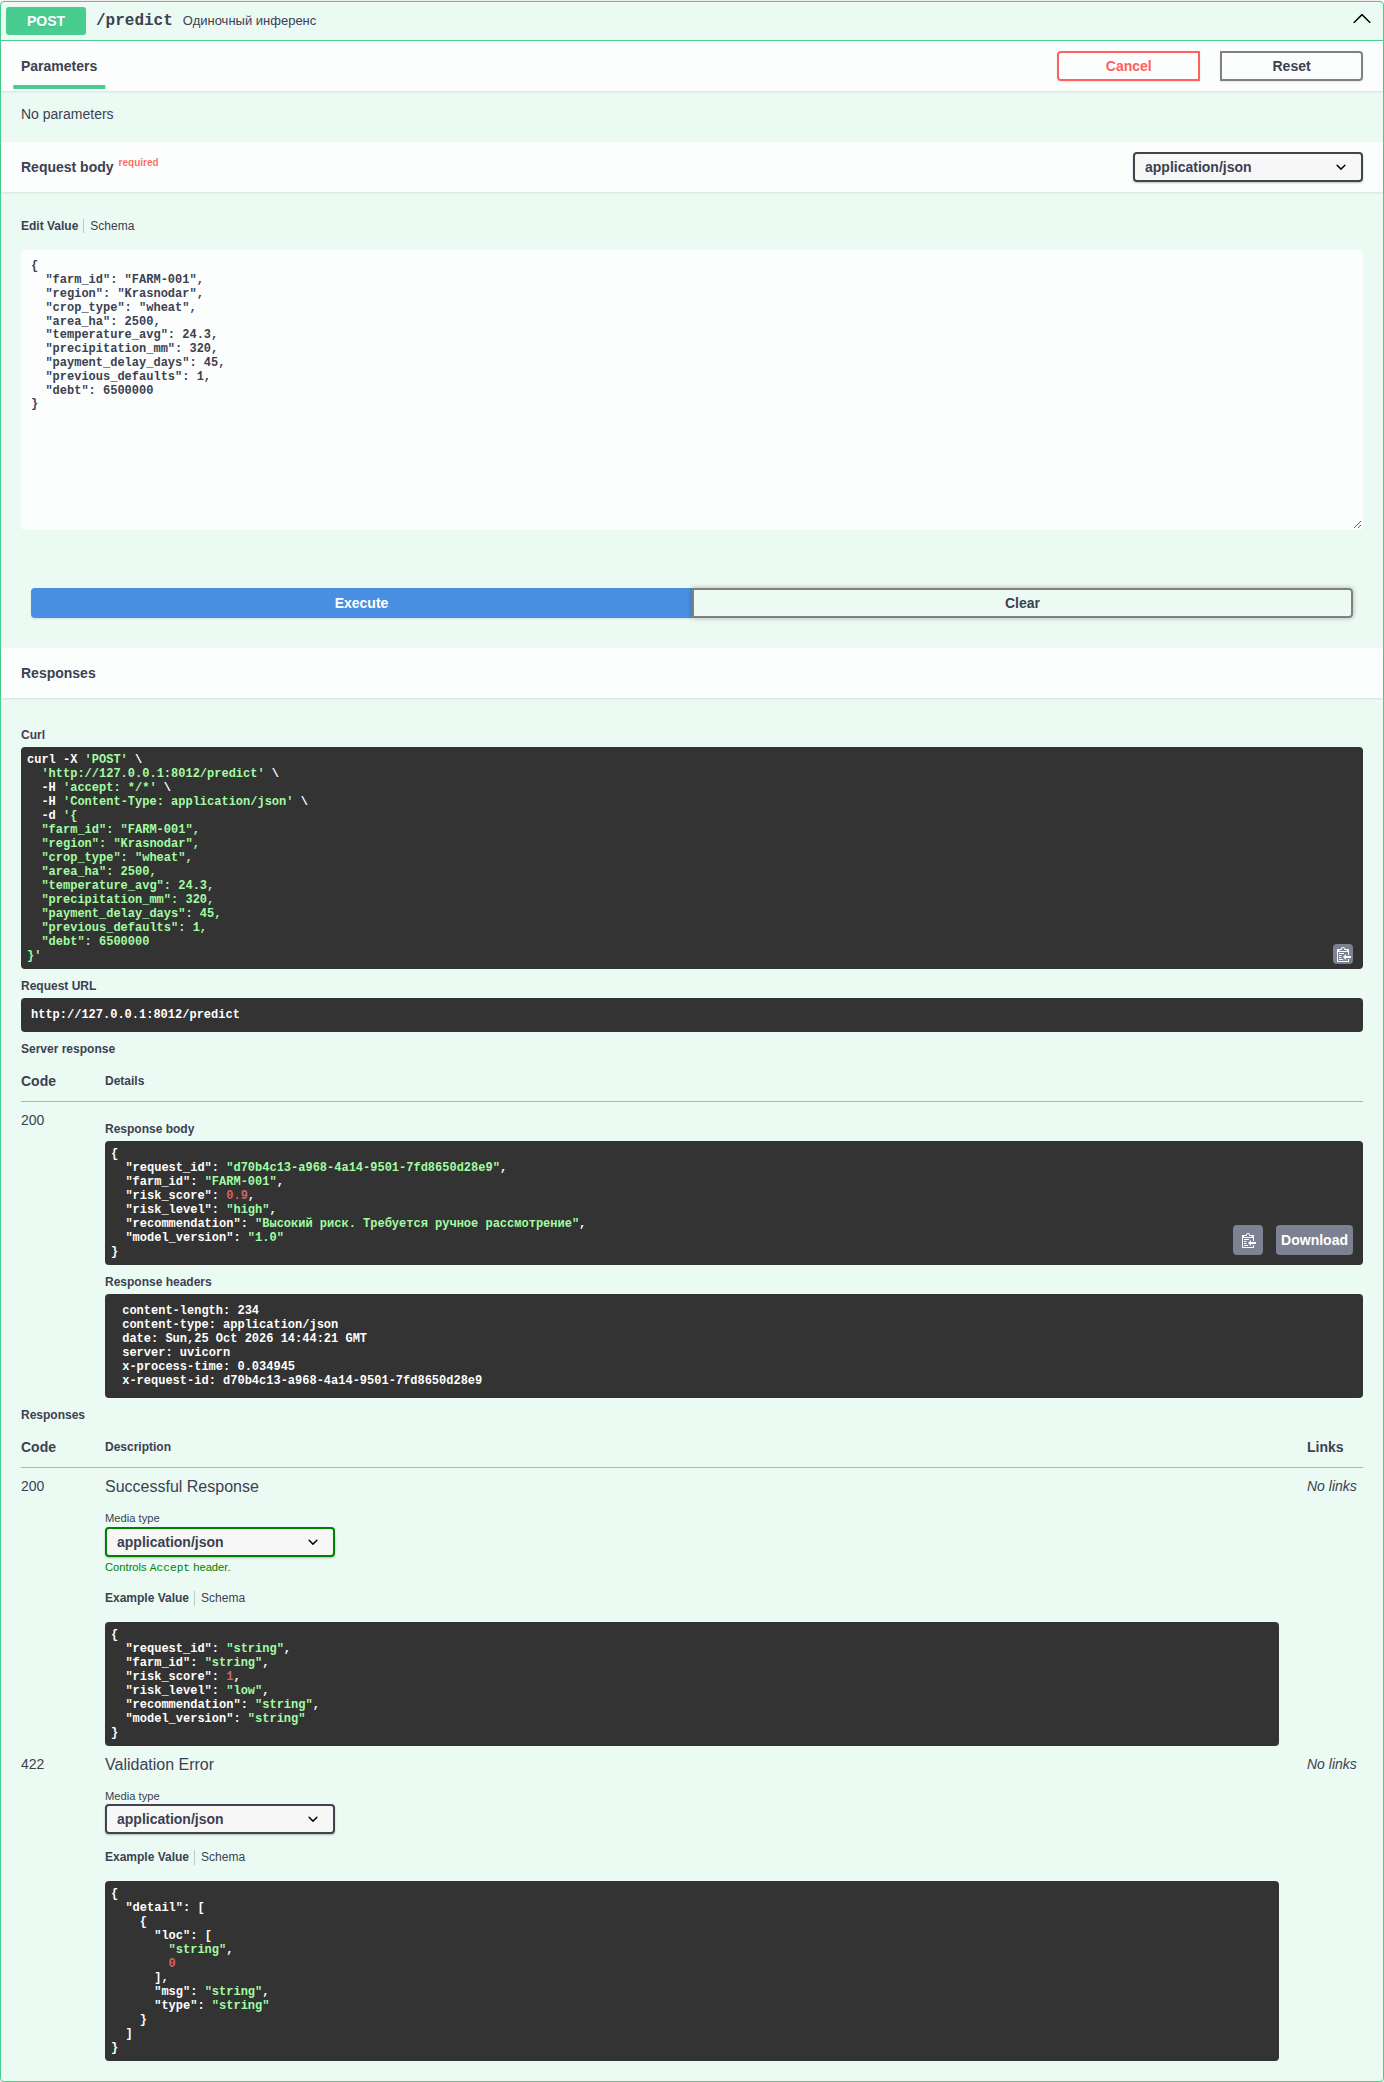
\includegraphics[width=\textwidth,height=.78\textheight,keepaspectratio]{predict.png}
  \caption{Успешный POST /predict}
\end{figure}

\begin{figure}[H]
  \centering
  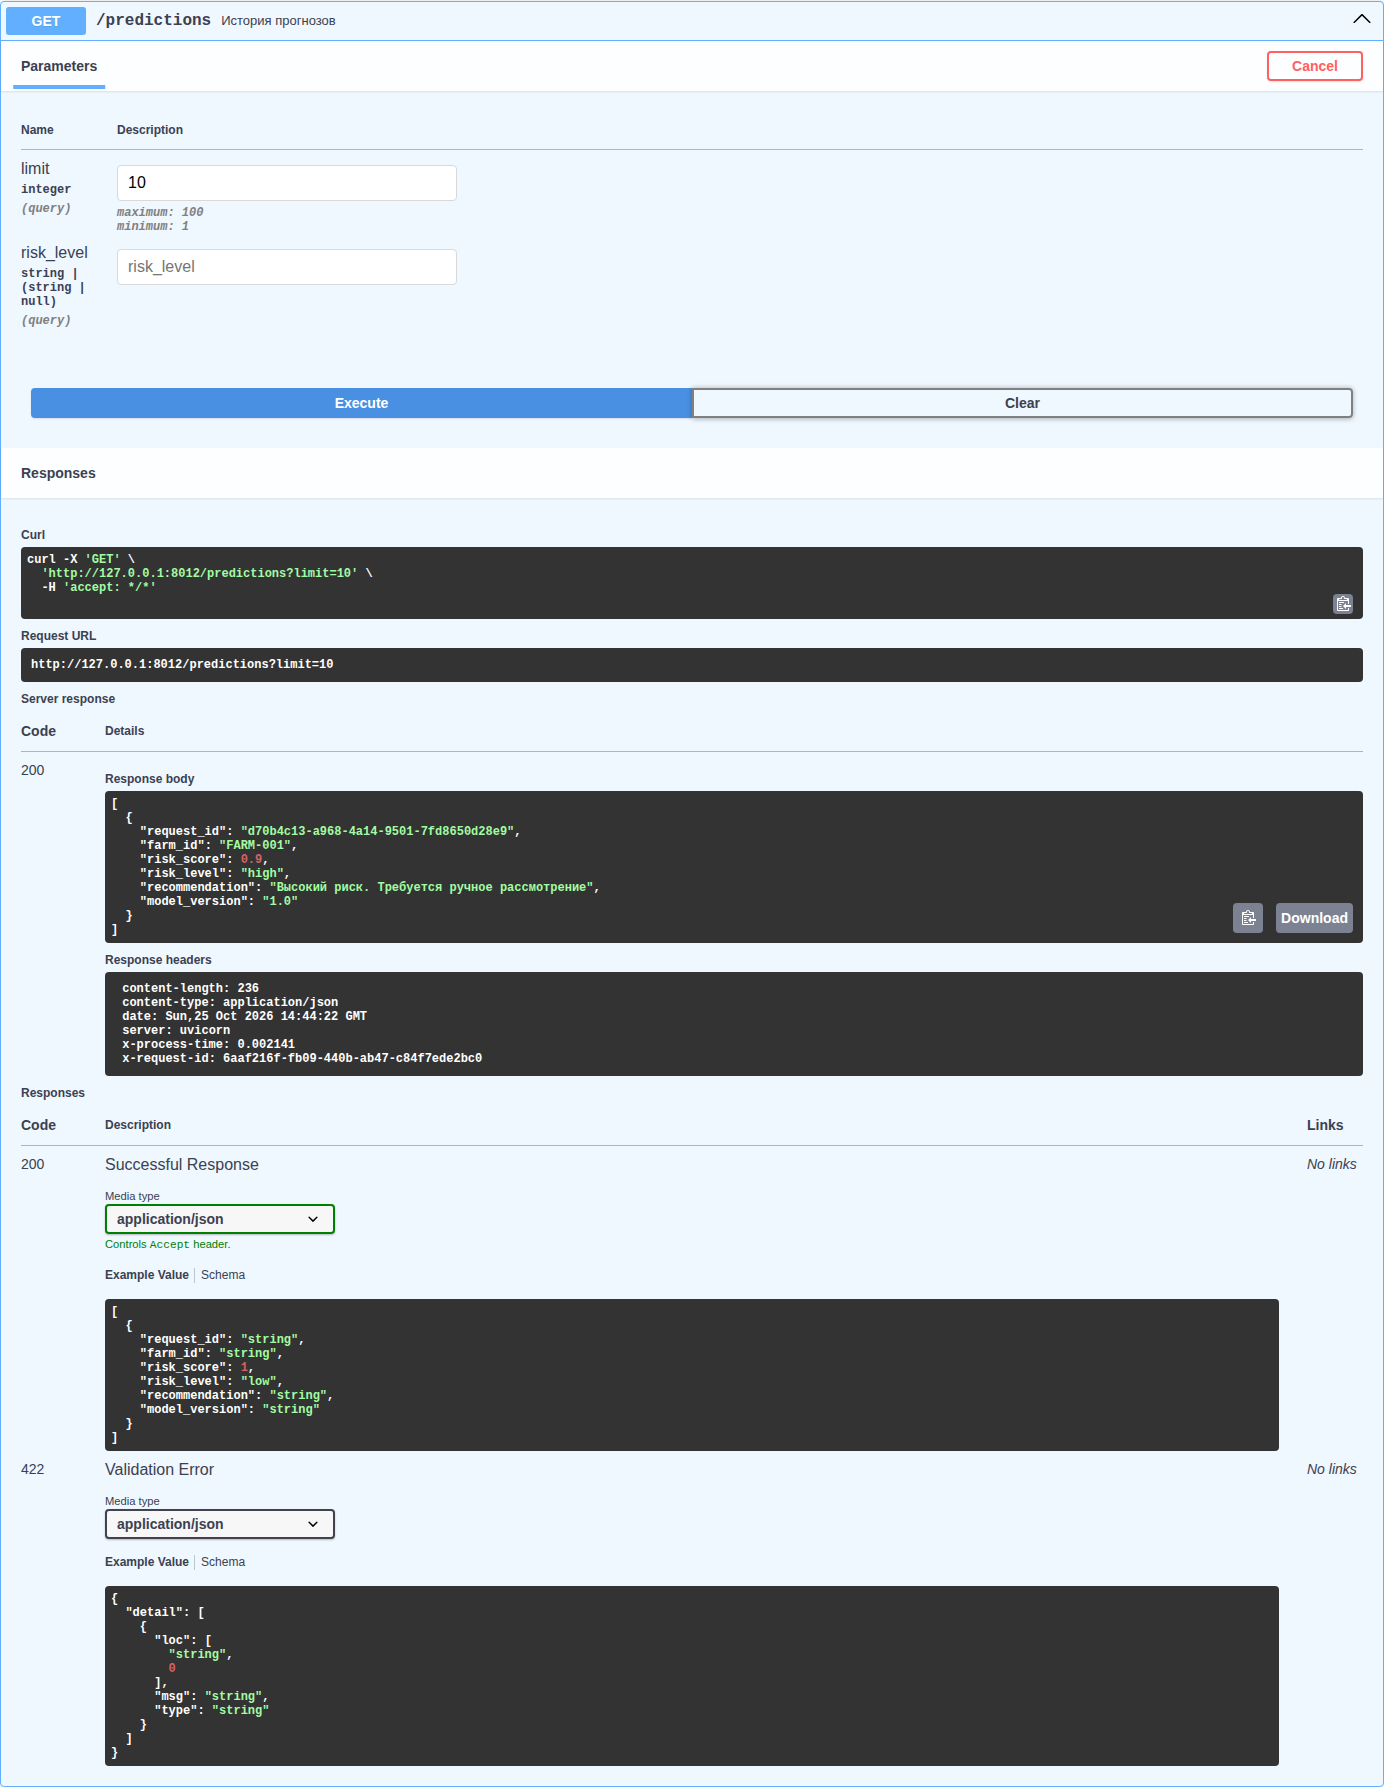
\includegraphics[width=\textwidth,height=.78\textheight,keepaspectratio]{predictions-sqlite.png}
  \caption{Чтение истории из SQLite}
\end{figure}

\subsection{Batching и backpressure}

Explicit batch обрабатывается одним вызовом модели и сохраняется одной
транзакцией. Dynamic batching принимает одиночные запросы, объединяет их в
worker и применяет backpressure при заполнении очереди.

\begin{figure}[H]
  \centering
  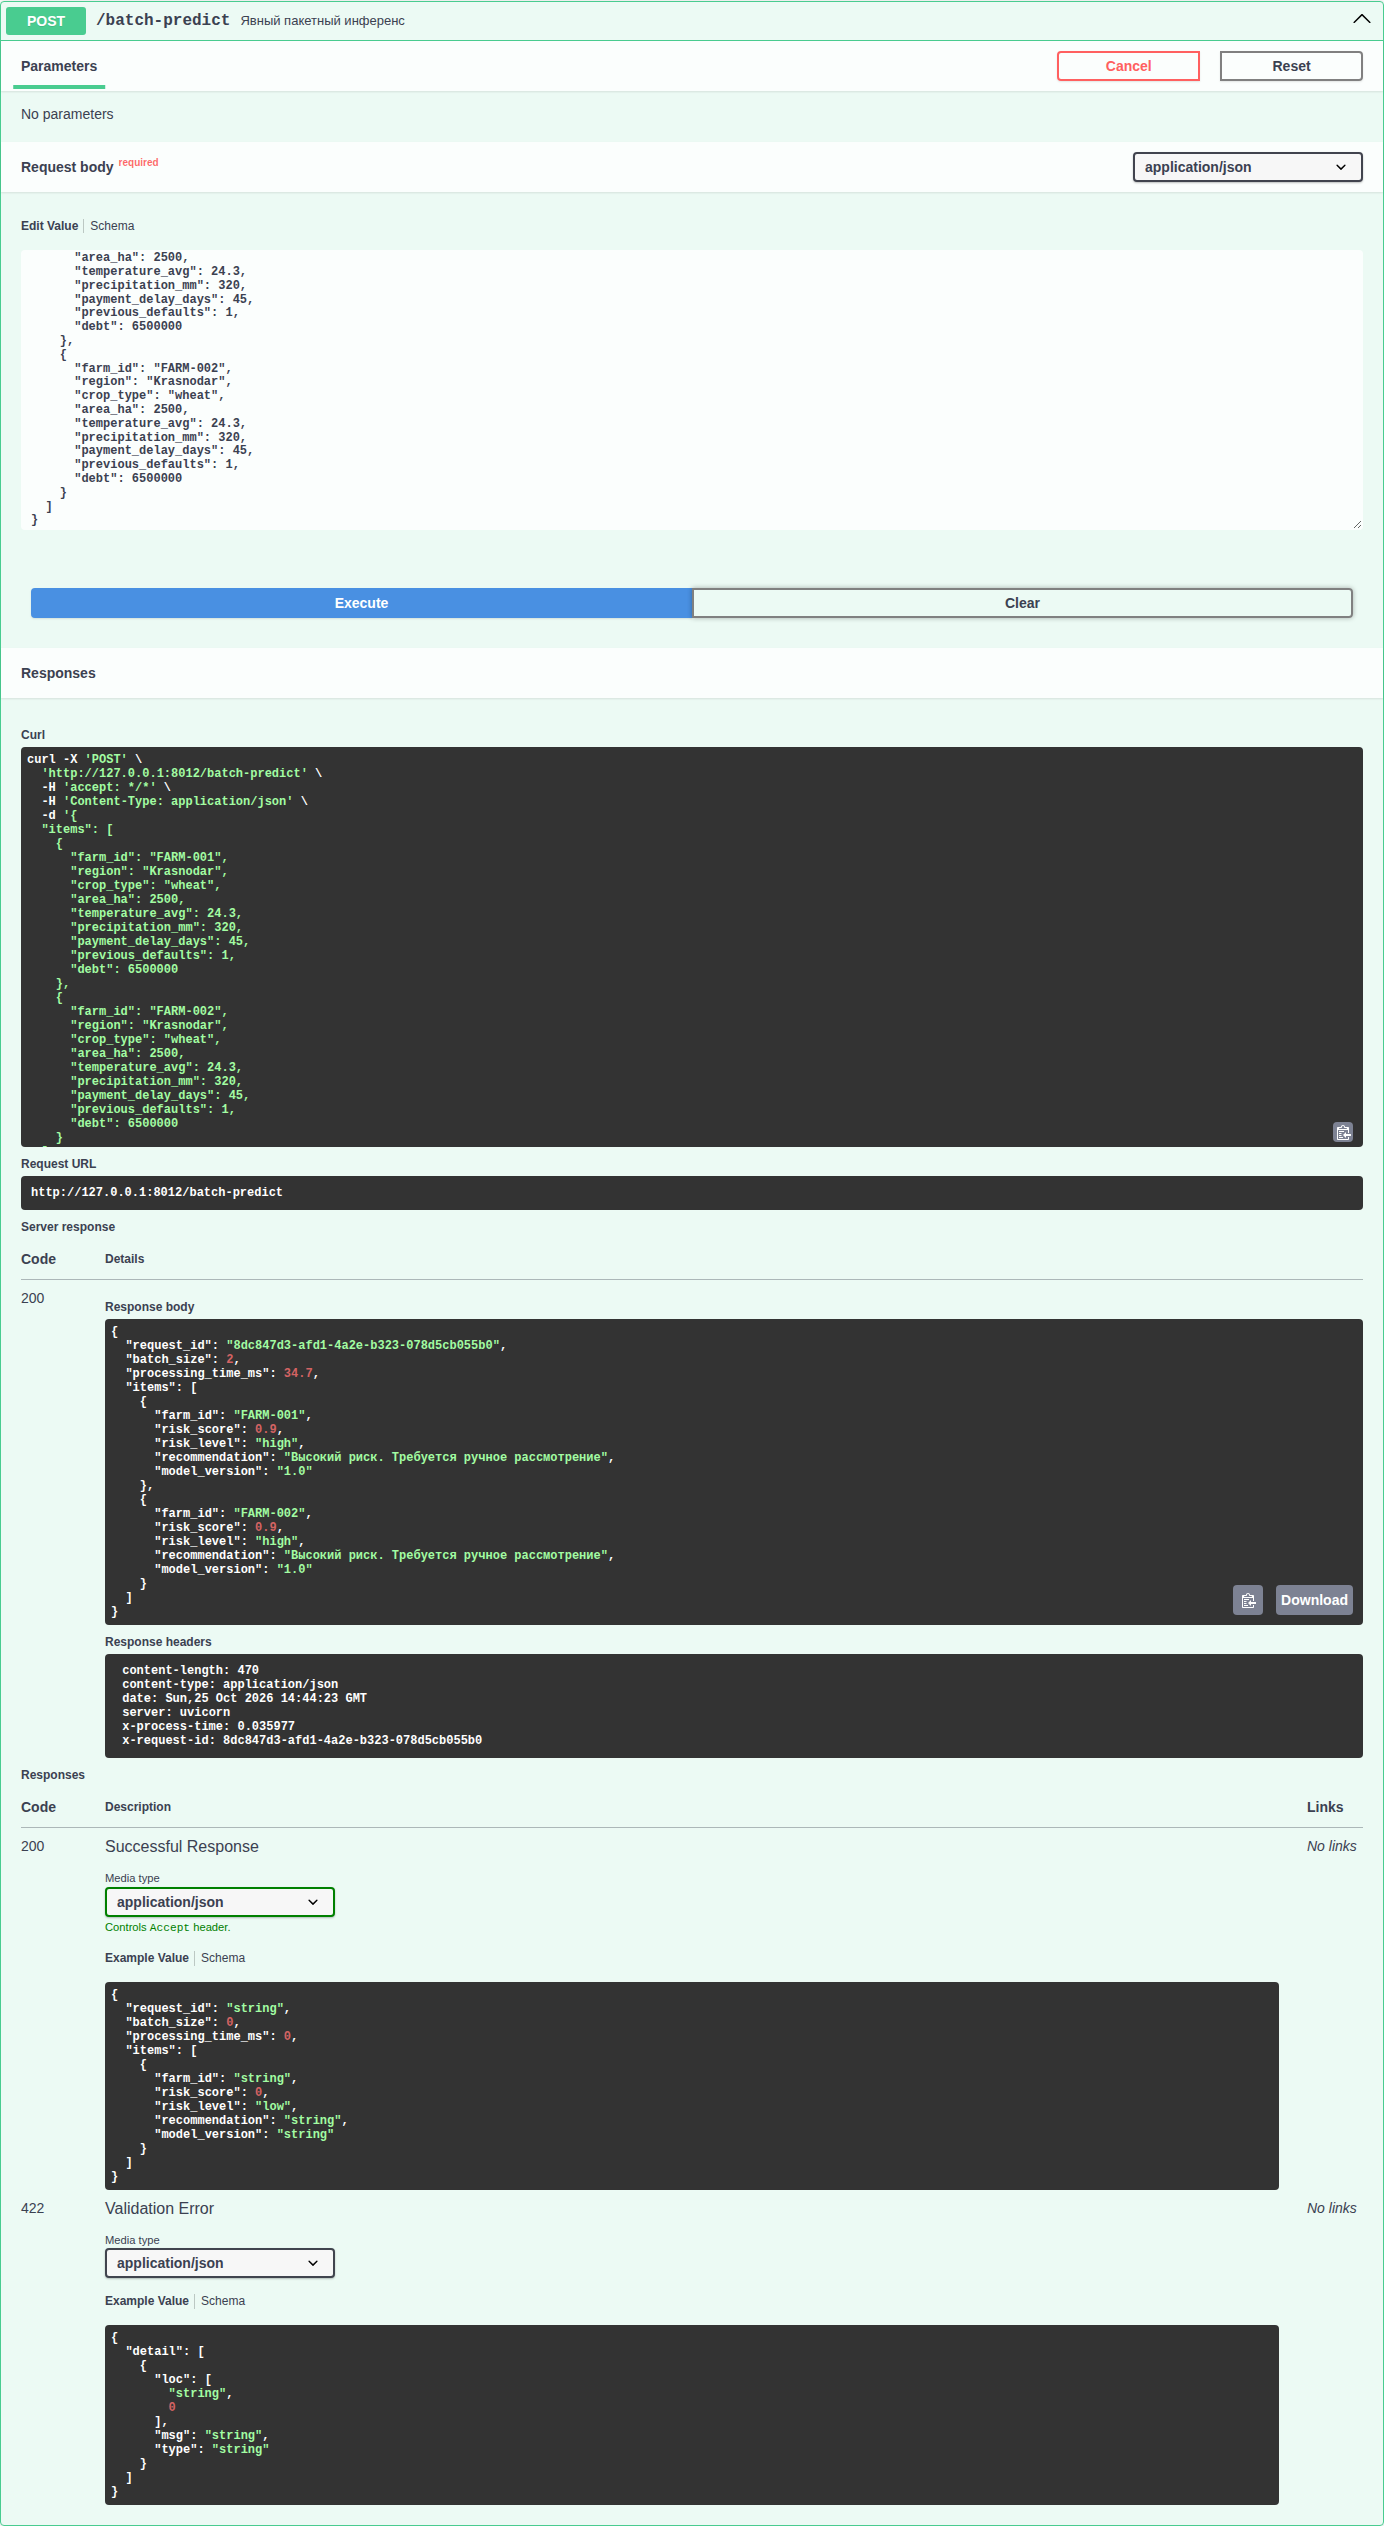
\includegraphics[width=\textwidth,height=.78\textheight,keepaspectratio]{batch-predict.png}
  \caption{Explicit batch inference}
\end{figure}

\begin{figure}[H]
  \centering
  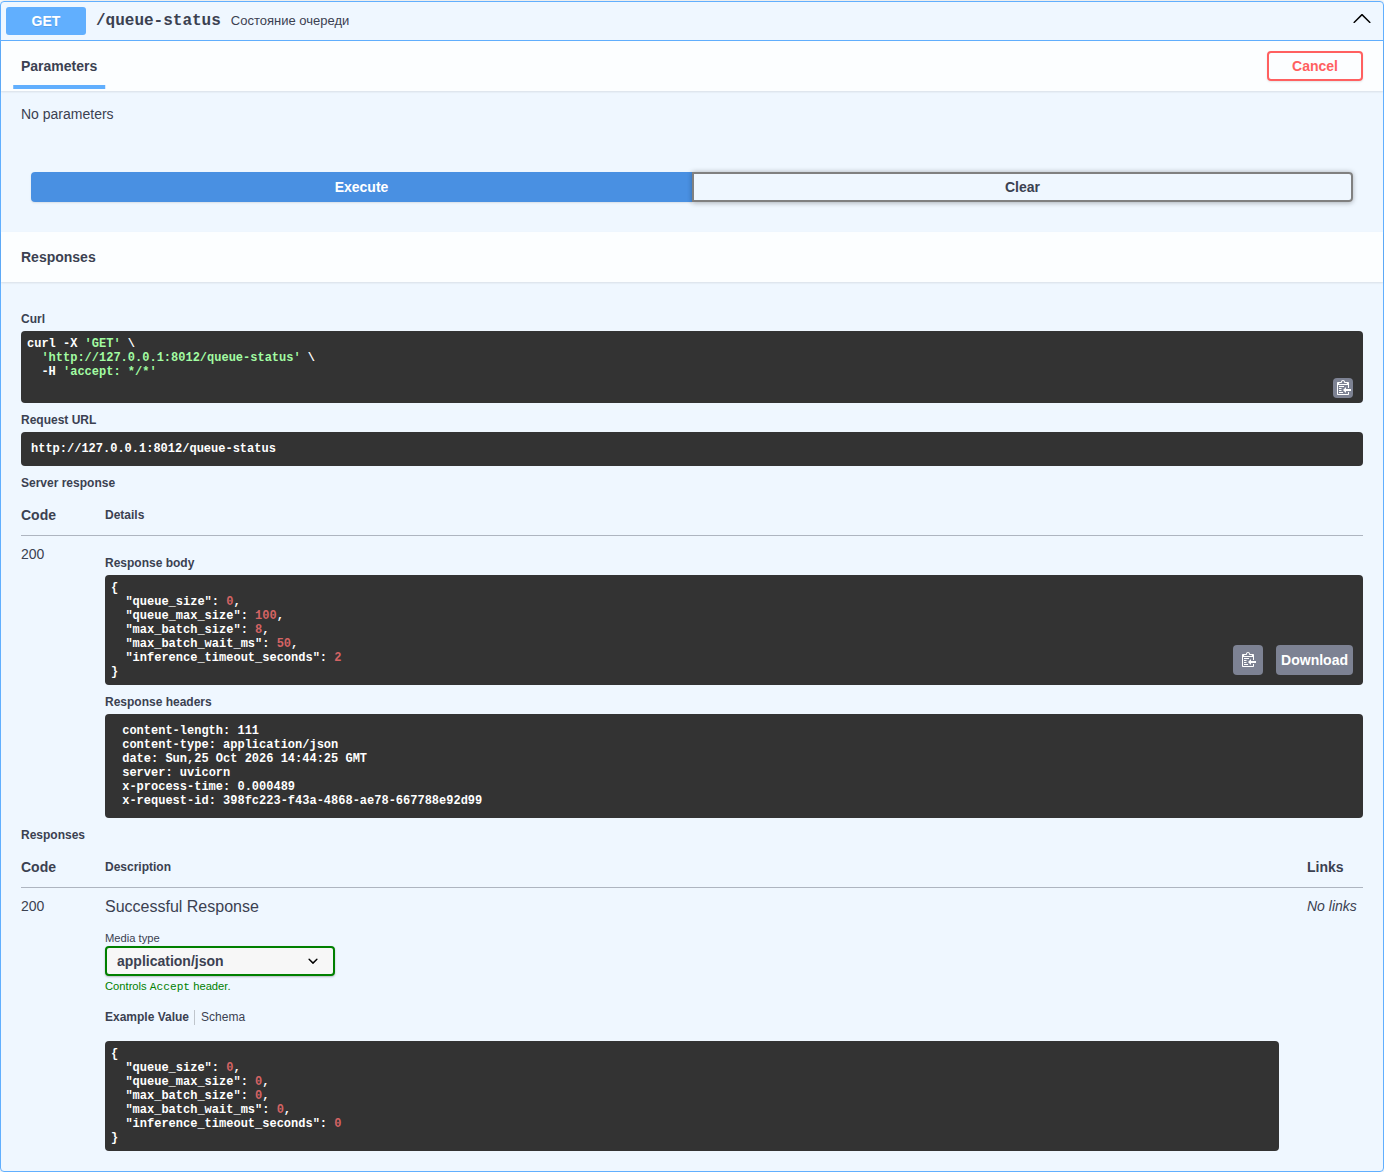
\includegraphics[width=\textwidth,height=.72\textheight,keepaspectratio]{queue-status.png}
  \caption{Состояние очереди dynamic batching}
\end{figure}

\subsection{Пагинация}

Endpoint использует \code{LIMIT}, \code{OFFSET} и отдельный \code{COUNT(*)},
возвращая ссылки на соседние страницы.

\begin{figure}[H]
  \centering
  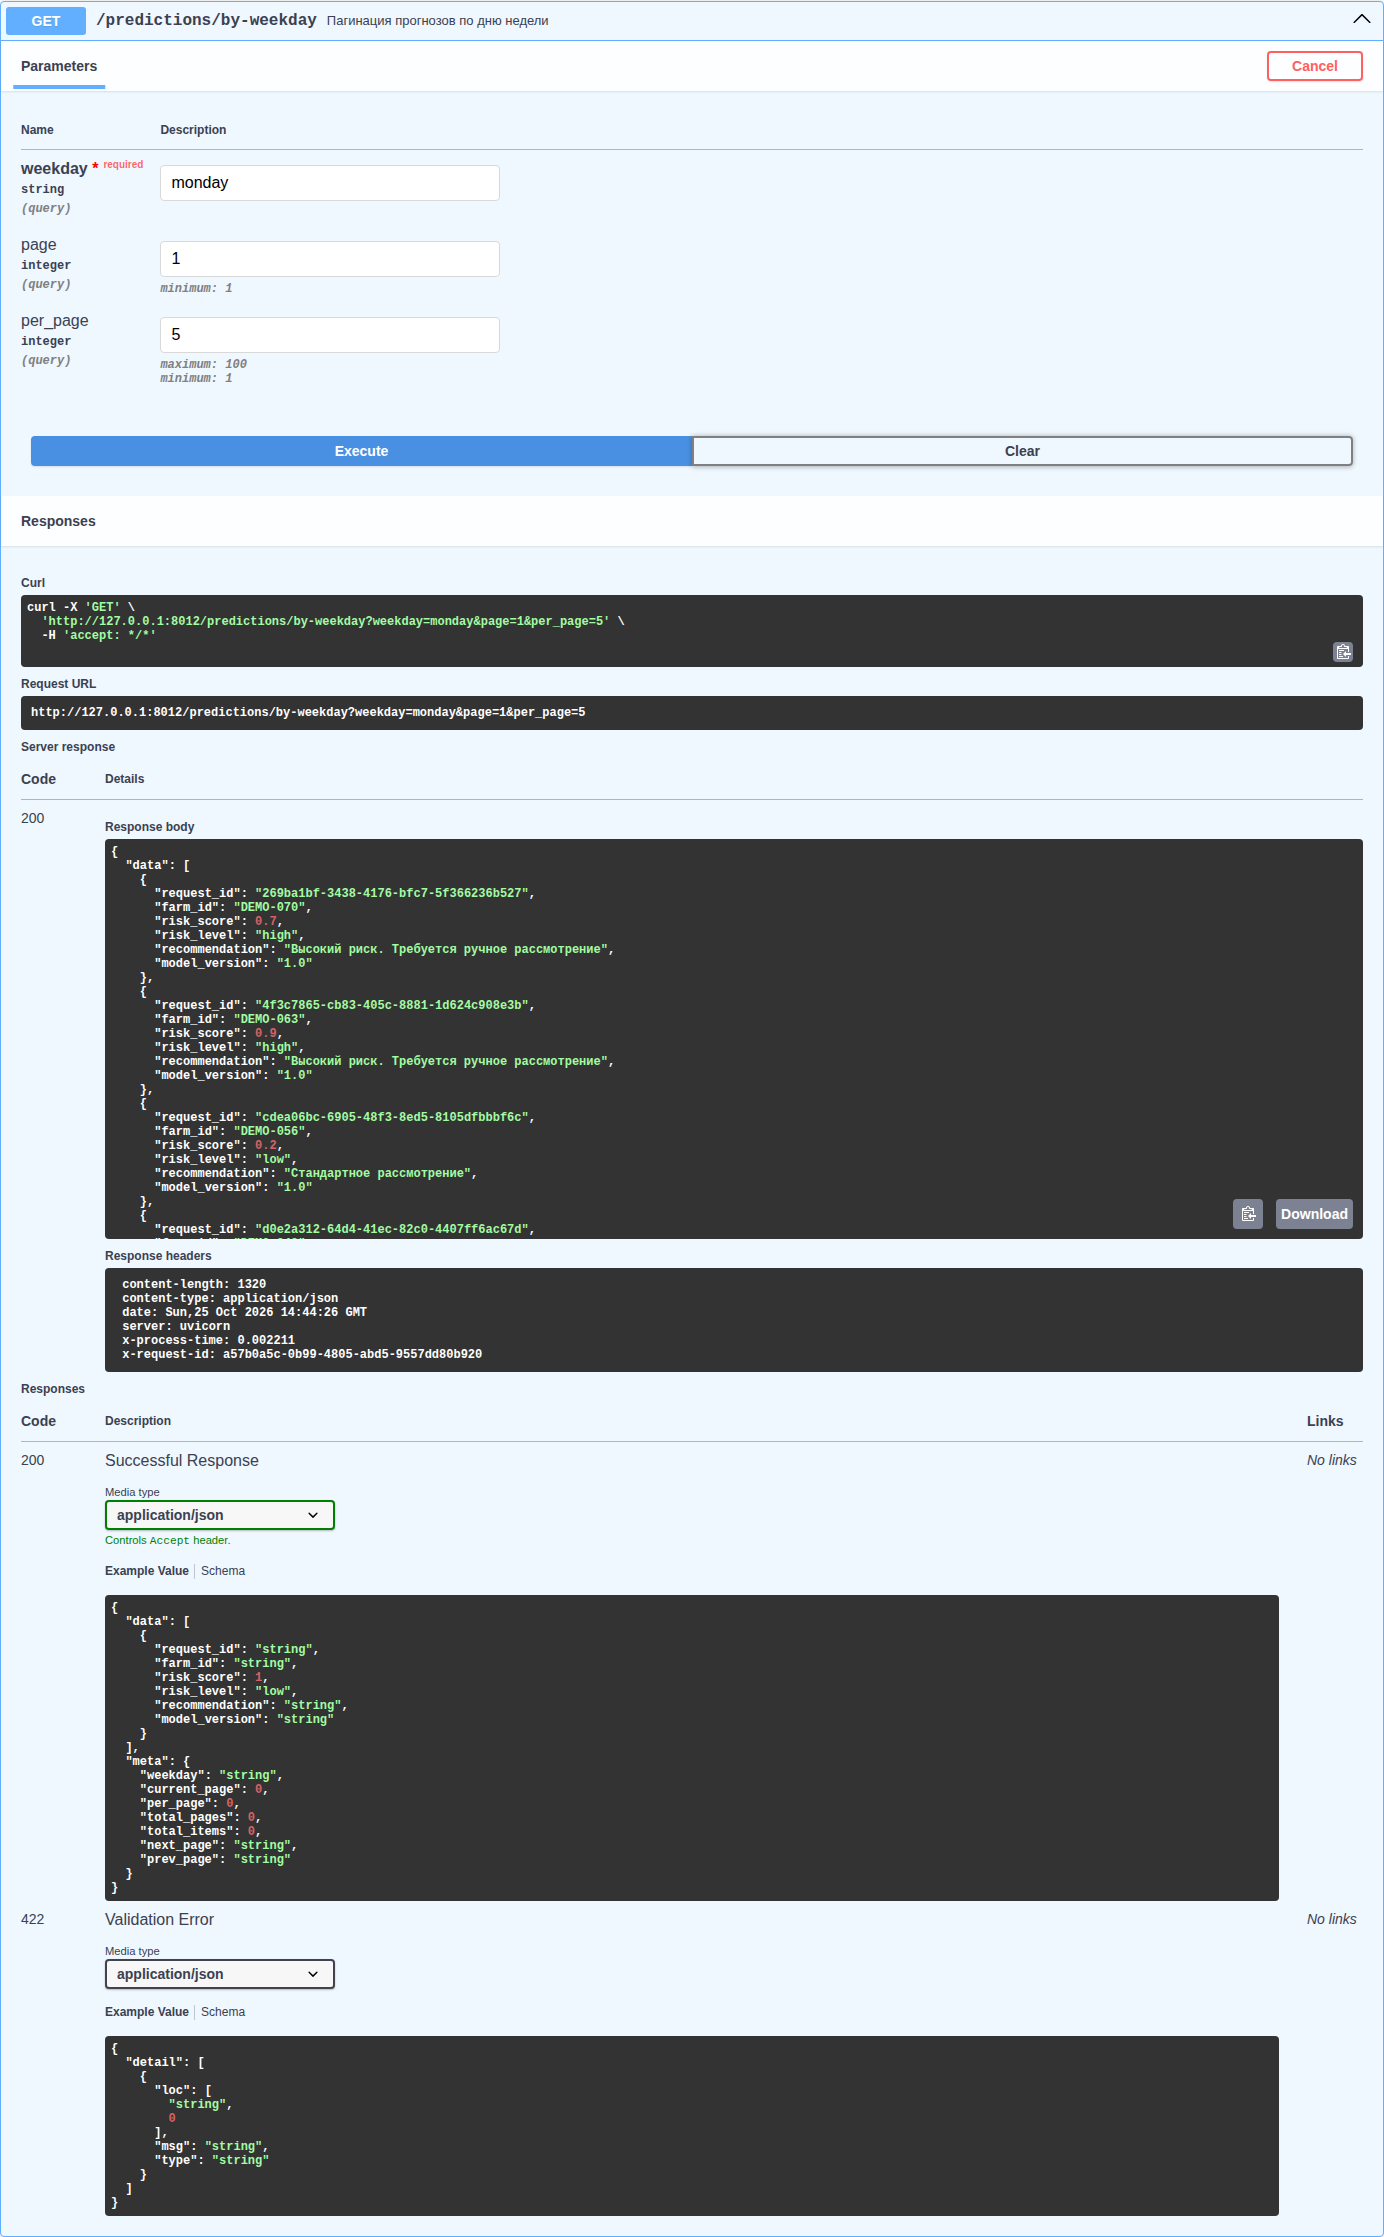
\includegraphics[width=\textwidth,height=.78\textheight,keepaspectratio]{weekday-pagination.png}
  \caption{Пагинация прогнозов за понедельник}
\end{figure}

\subsection{Подключение LLM}

В \code{/predict-with-llm} сначала выполняется детерминированный скоринг. Во
внешний сервис передаются только результат, рекомендация и версия модели, без
\code{farm\_id} и финансовых признаков. LLM формирует пояснение, но не изменяет
\code{risk\_score} и \code{risk\_level}.

\begin{figure}[H]
  \centering
  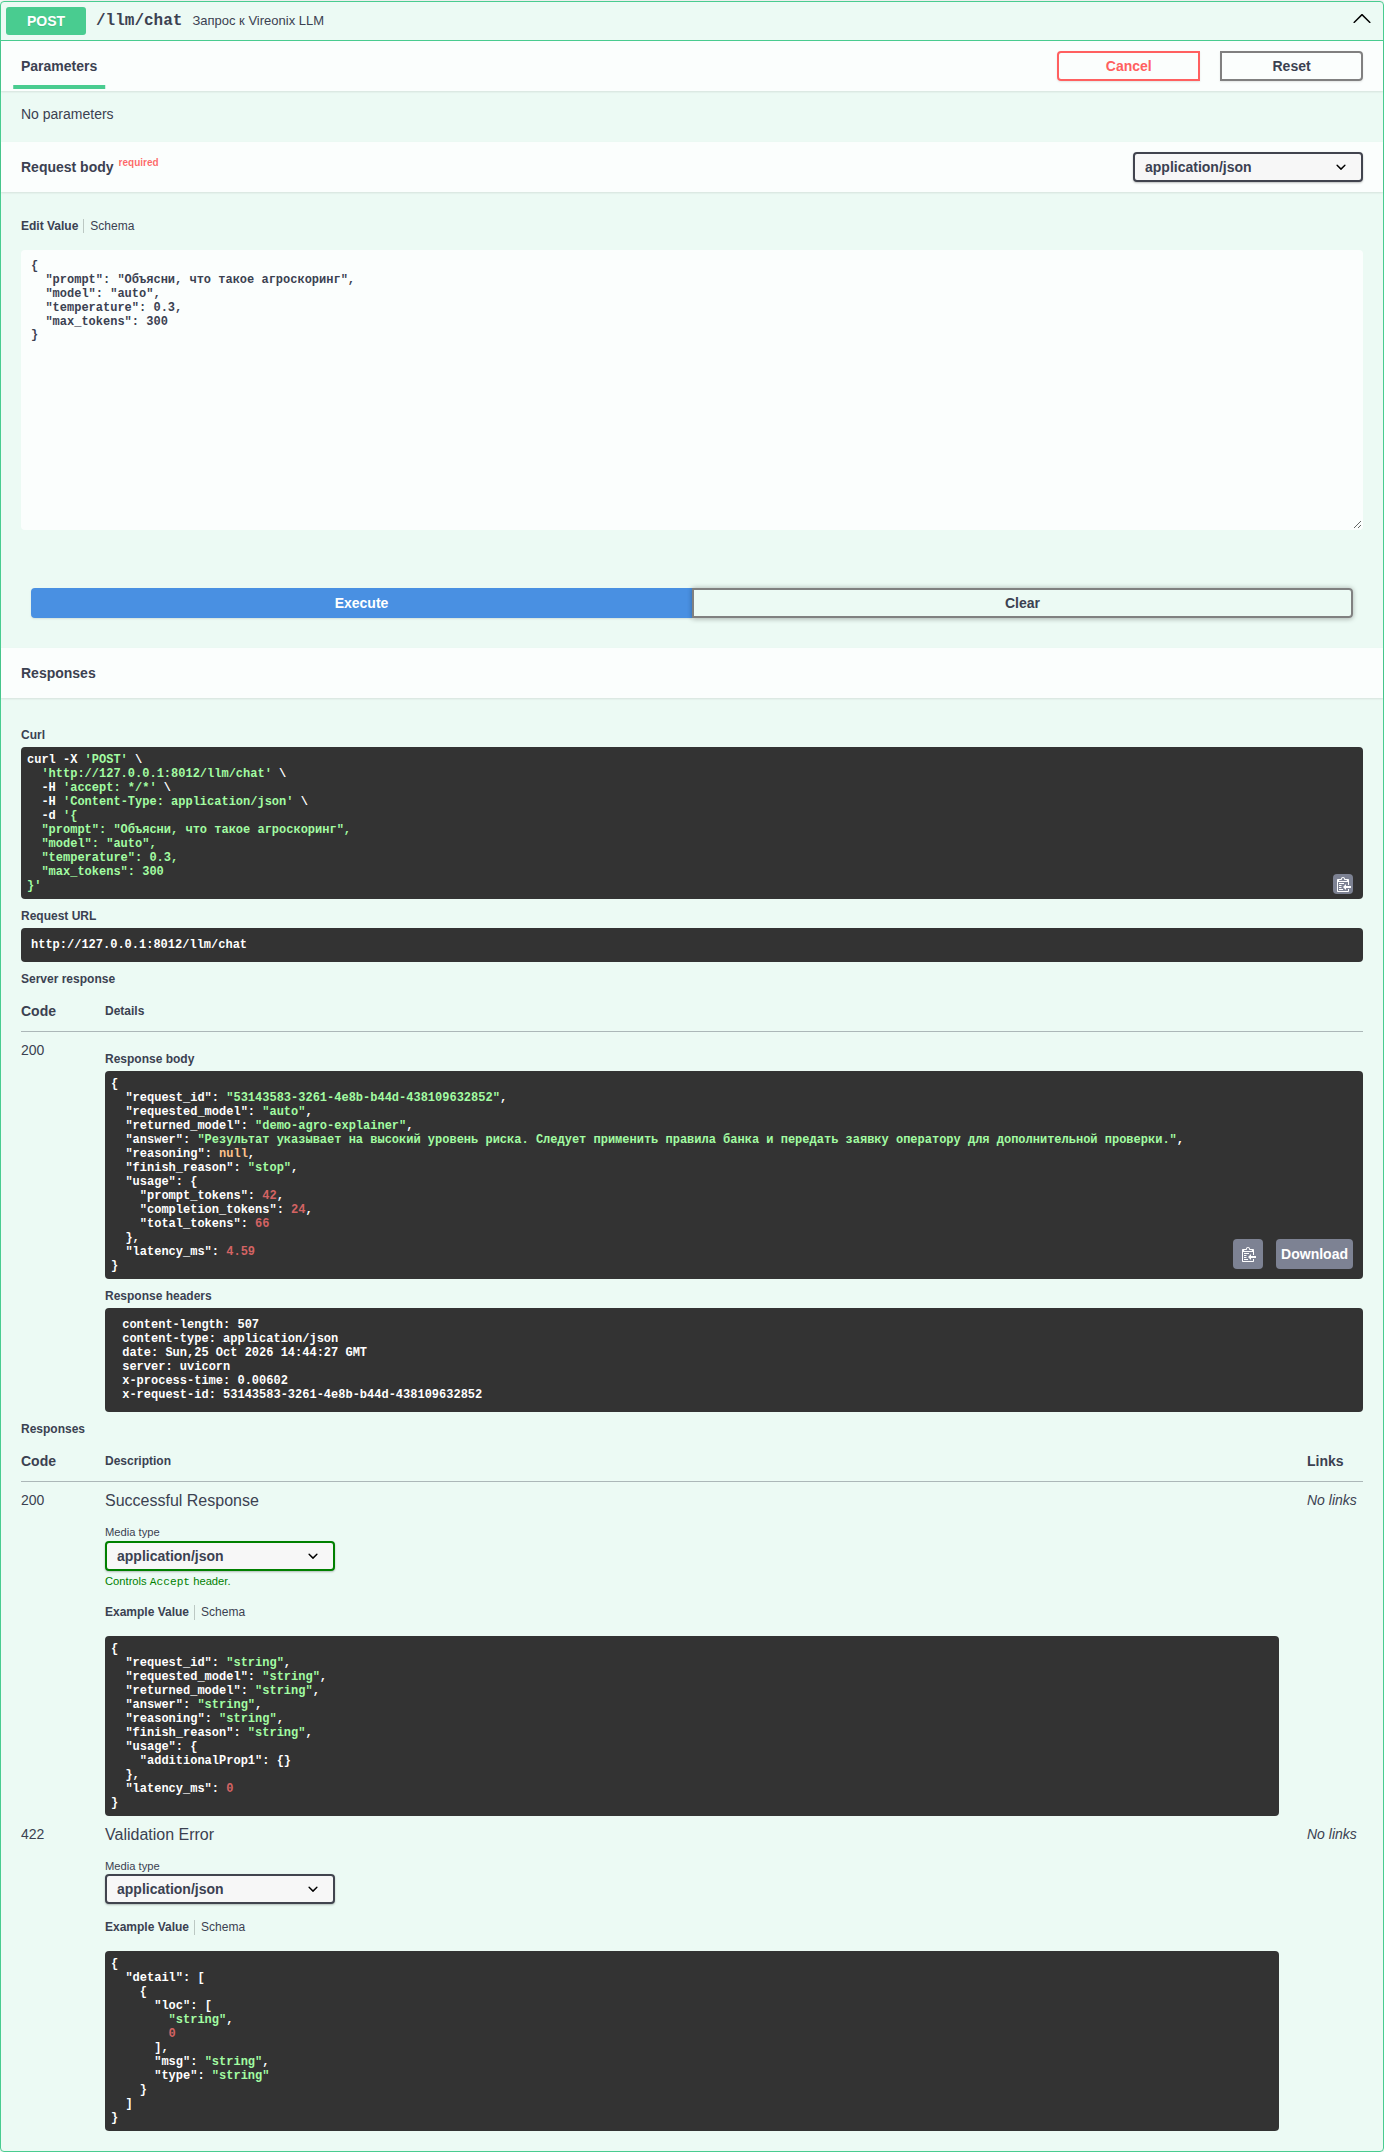
\includegraphics[width=\textwidth,height=.78\textheight,keepaspectratio]{llm-chat.png}
  \caption{Учебный запрос к LLM}
\end{figure}

\begin{figure}[H]
  \centering
  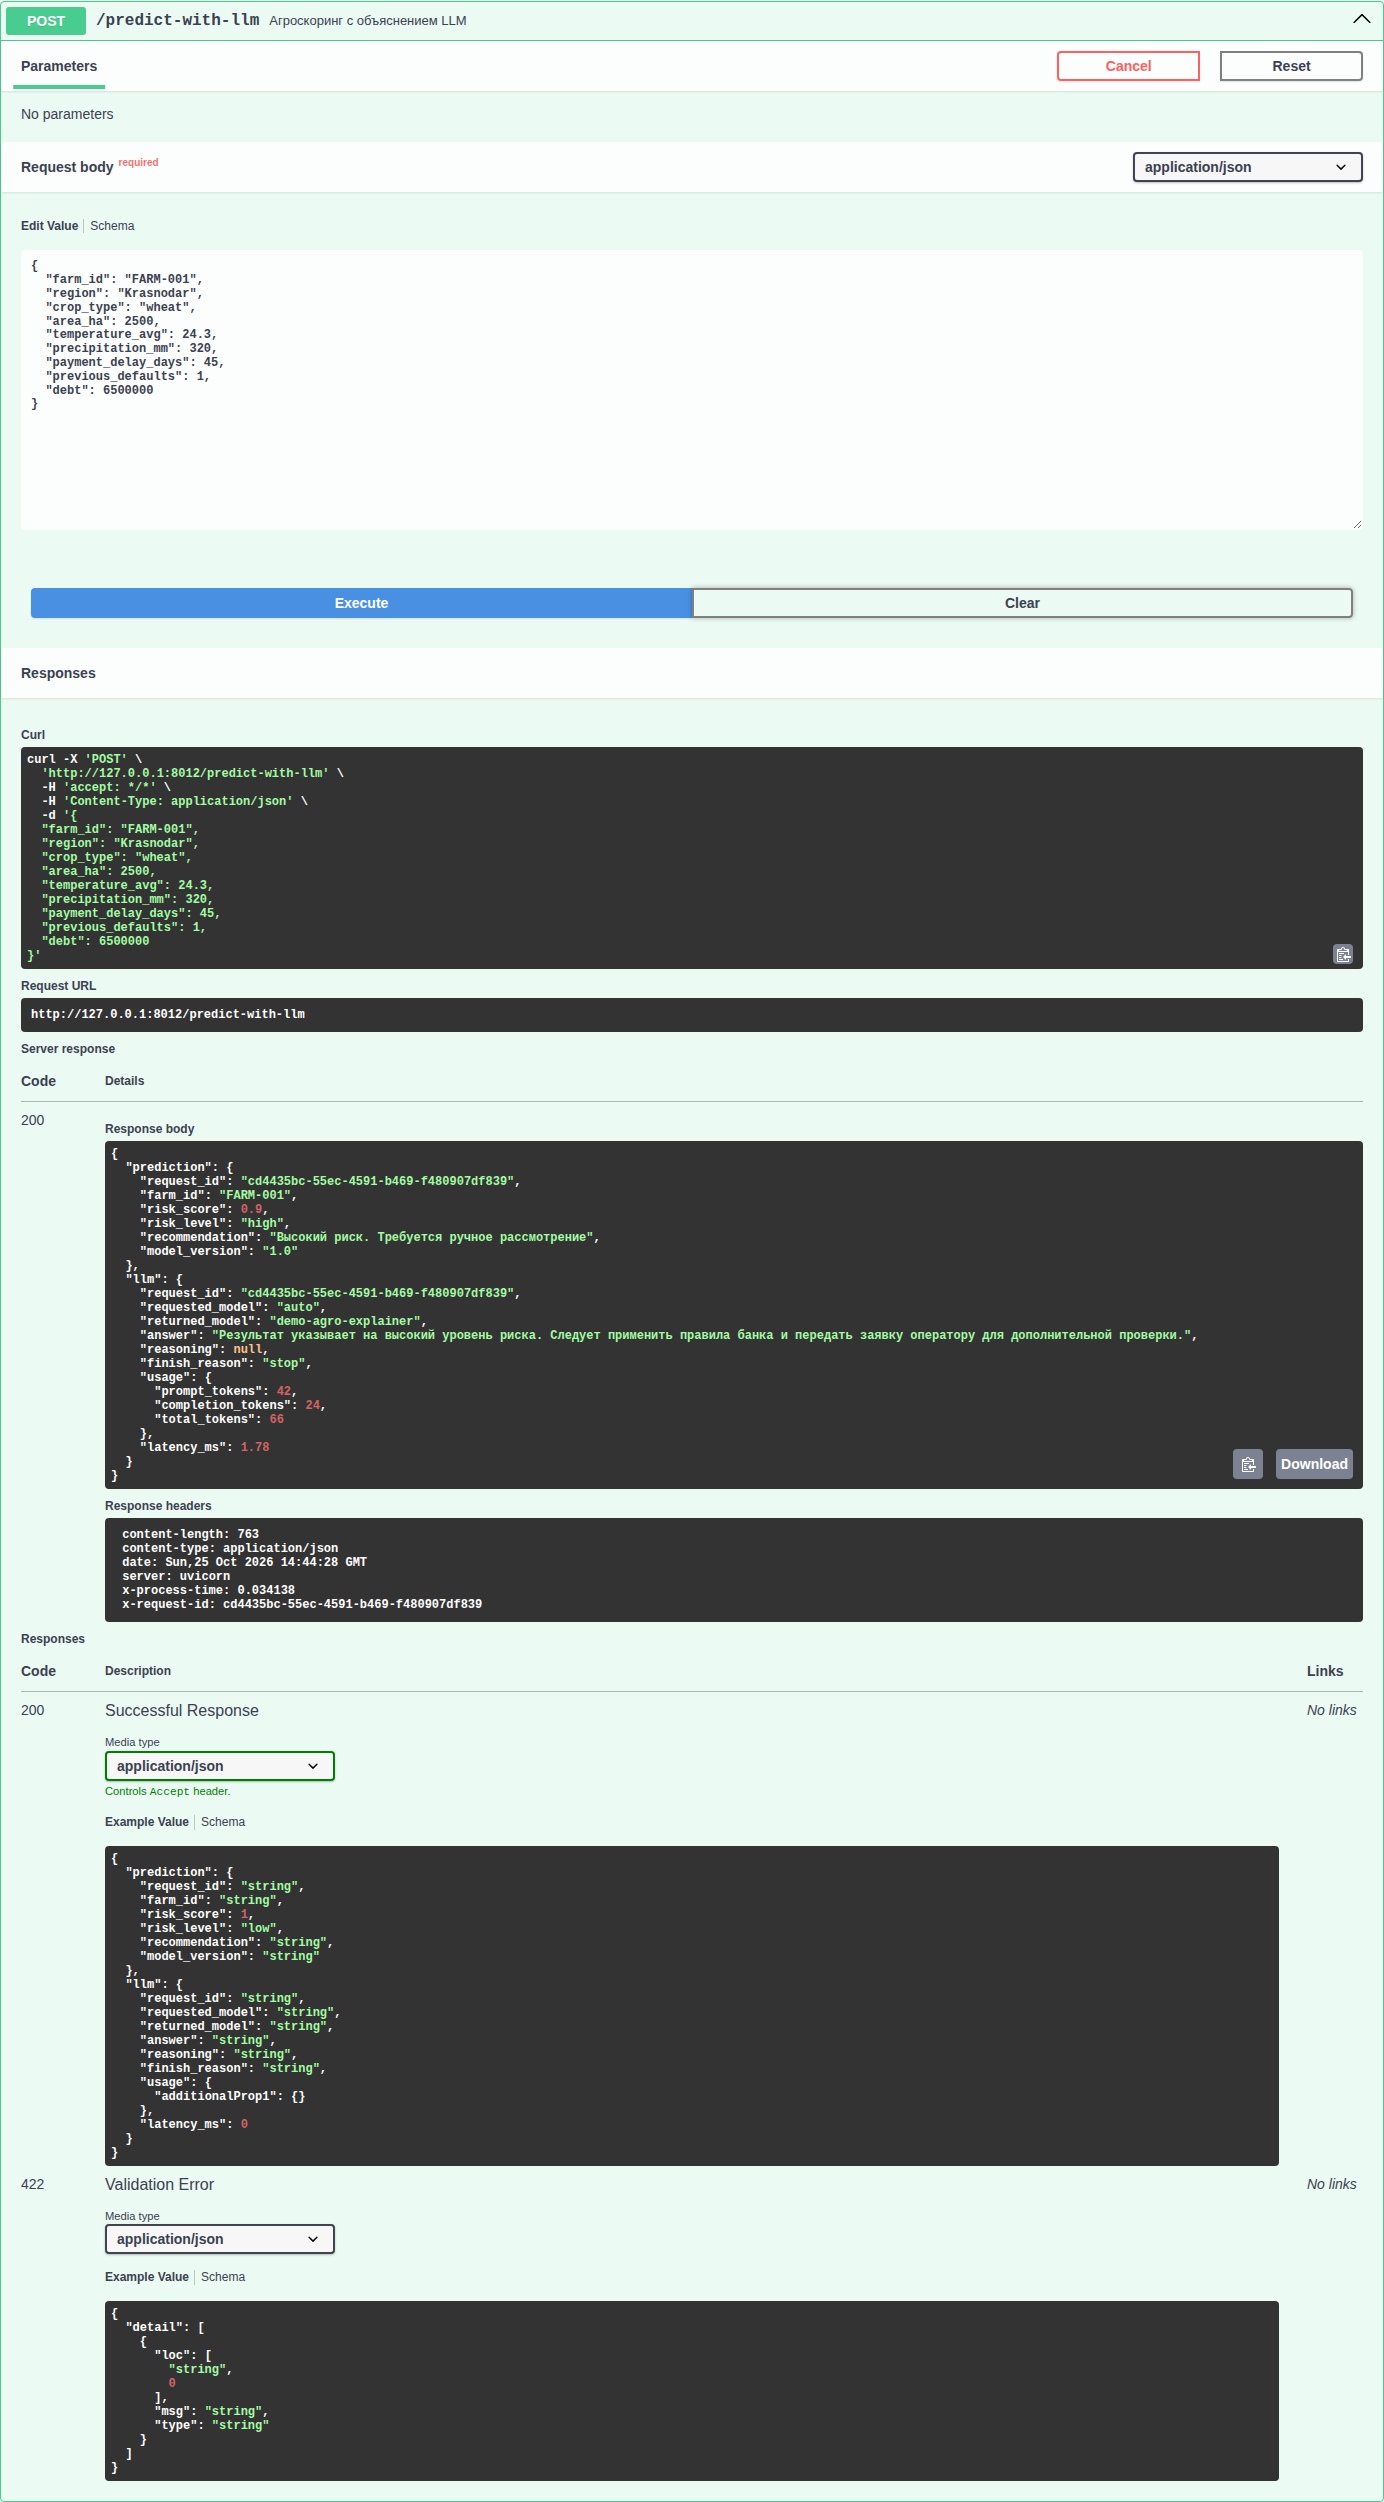
\includegraphics[width=\textwidth,height=.78\textheight,keepaspectratio]{predict-with-llm.png}
  \caption{Скоринг с текстовым объяснением}
\end{figure}

Приложение по умолчанию настроено на \url{https://vireonix.ai/v1}. Во время
подготовки отчёта провайдер отвечал кодом 502 и сообщал о временной
недоступности. Поэтому успешные скриншоты получены через локальный
OpenAI-совместимый демонстрационный провайдер. Обработка ошибок реального
провайдера проверена автоматическими тестами.

\section{Тестирование}

\begin{longtable}{>{\raggedleft\arraybackslash}p{.5cm}
                  >{\raggedright\arraybackslash}p{6.4cm}
                  >{\centering\arraybackslash}p{2.2cm}
                  >{\centering\arraybackslash}p{2.2cm}
                  >{\raggedright\arraybackslash}p{2.1cm}}
  \caption{Обязательные тест-кейсы}\label{tab:tests}\\
  \toprule
  \textbf{№} & \textbf{Запрос} & \textbf{Ожидаемый код} &
  \textbf{Полученный код} & \textbf{Результат} \\
  \midrule\endfirsthead
  \toprule
  \textbf{№} & \textbf{Запрос} & \textbf{Ожидаемый код} &
  \textbf{Полученный код} & \textbf{Результат} \\
  \midrule\endhead
  \bottomrule\endfoot
  1 & \code{GET /health} & 200 & 200 & Пройден \\
  2 & Корректный \code{POST /predict} & 200 & 200 & Пройден \\
  3 & \code{area\_ha = -100} & 422 & 422 & Пройден \\
  4 & Неизвестный регион & 400 & 400 & Пройден \\
  5 & Существующий \code{request\_id} & 200 & 200 & Пройден \\
  6 & Неизвестный \code{request\_id} & 404 & 404 & Пройден \\
  7 & Корректный \code{POST /batch-predict} & 200 & 200 & Пройден \\
  8 & Batch больше максимума & 422 & 422 & Пройден \\
  9 & \code{POST /predict-queued} & 200 & 200 & Пройден \\
  10 & Переполненная очередь & 429 & 429 & Пройден \\
  11 & Пагинация, первая страница & 200 & 200 & Пройден \\
  12 & \code{page = -1} & 422 & 422 & Пройден \\
  13 & Неизвестный weekday & 400 & 400 & Пройден \\
  14 & Корректный \code{POST /llm/chat} & 200 & 200 & Пройден \\
  15 & Ошибка LLM-провайдера & 502/503/504 & 502/503/504 & Пройден \\
  16 & Корректный \code{POST /predict-with-llm} & 200 & 200 & Пройден \\
\end{longtable}

Всего выполнено 28 автоматических тестов. Дополнительно проверены параллельные
queued-запросы, конфликт 409 для batch, timeout, недоступность модели,
сквозной request ID, ответ 500, фильтрация, OpenAPI и отсутствие
конфиденциальных данных в LLM-промпте.

\section{Анализ API-контракта}

\begin{longtable}{>{\ttfamily\raggedright\arraybackslash}p{3.5cm}
                  >{\centering\arraybackslash}p{1.2cm}
                  >{\raggedright\arraybackslash}p{2.7cm}
                  >{\raggedright\arraybackslash}p{3.1cm}
                  >{\centering\arraybackslash}p{1.3cm}
                  >{\raggedright\arraybackslash}p{2.5cm}}
  \caption{Основной API-контракт}\label{tab:contract}\\
  \toprule
  \normalfont\textbf{Endpoint} & \textbf{Метод} & \textbf{Вход} &
  \textbf{Выход} & \textbf{Успех} & \textbf{Ошибки} \\
  \midrule\endfirsthead
  \toprule
  \normalfont\textbf{Endpoint} & \textbf{Метод} & \textbf{Вход} &
  \textbf{Выход} & \textbf{Успех} & \textbf{Ошибки} \\
  \midrule\endhead
  \bottomrule\endfoot
  /health & \normalfont GET & \normalfont --- & HealthResponse & 200 & \normalfont 500 \\
  /predict & \normalfont POST & FarmRequest & PredictionResponse & 200 & \normalfont 400, 422, 503, 504 \\
  /batch-predict & \normalfont POST & BatchRequest & BatchPredictionResponse & 200 & \normalfont 400, 422, 503, 504 \\
  /predict-queued & \normalfont POST & FarmRequest & PredictionResponse & 200 & \normalfont 400, 422, 429, 503, 504 \\
  /predictions & \normalfont GET & \normalfont query & PredictionResponse[] & 200 & \normalfont 400, 422, 503 \\
  /predictions/by-weekday & \normalfont GET & \normalfont weekday, page, per\_page & PaginatedResponse & 200 & \normalfont 400, 404, 422, 503 \\
  /llm/chat & \normalfont POST & LLMChatRequest & LLMChatResponse & 200 & \normalfont 422, 502, 503, 504 \\
  /predict-with-llm & \normalfont POST & FarmRequest & PredictWithLLMResponse & 200 & \normalfont 400, 422, 502, 503, 504 \\
\end{longtable}

\section{Ответы на контрольные вопросы}

\textbf{Почему блокирующий \code{sqlite3.execute()} нежелателен?}
Он занимает поток event loop до завершения операции, поэтому этот worker не
может обслуживать другие соединения. \code{aiosqlite} позволяет ожидать
операцию через \code{await}, не блокируя обработку остальных запросов.

\textbf{Почему один \code{executemany()} лучше восьми \code{INSERT + COMMIT}?}
Уменьшается число дисковых синхронизаций и транзакционных накладных расходов,
растёт throughput, а весь batch сохраняется атомарно.

\textbf{Что произойдёт с неограниченной очередью?}
При перегрузке очередь будет расти быстрее, чем модель обрабатывает запросы.
Это приведёт к росту памяти и latency вплоть до падения процесса. Ограниченная
очередь создаёт backpressure и возвращает 429 до исчерпания ресурсов.

\section{Вывод}

Сервис дополнен трассировкой, постоянным асинхронным хранилищем, управлением
нагрузкой, пакетным инференсом, timeout и наблюдаемостью. Детерминированный
скоринг отделён от LLM: модель рассчитывает риск, а LLM формирует только
объяснение. Это сохраняет воспроизводимость решения и снижает риск утечки
данных.

\end{document}
